\section{Algoritmo 3: Numba en Python}
\label{sec:algo3_numba}

\subsection{Implementación y Warm-up}
Se implementó en Python el paralelismo de datos sobre la multiplicación densa de $N \times N$ ($N=2048$) empleando Numba con el decorador \texttt{@njit(parallel=True)} y la directiva \texttt{prange} en el bucle exterior. Para evitar incluir el tiempo de compilación JIT e inferencia de tipos en las mediciones, se efectuó una llamada previa de precalentamiento (\emph{warm-up}) con matrices de $64 \times 64$. El control de hilos se realizó dinámicamente mediante \texttt{numba.set\_num\_threads(p)}. El \emph{checksum} verificado fue exactamente $172.331627$, idéntico al de las versiones en C++.

\begin{figure}[htbp]
    \centering
    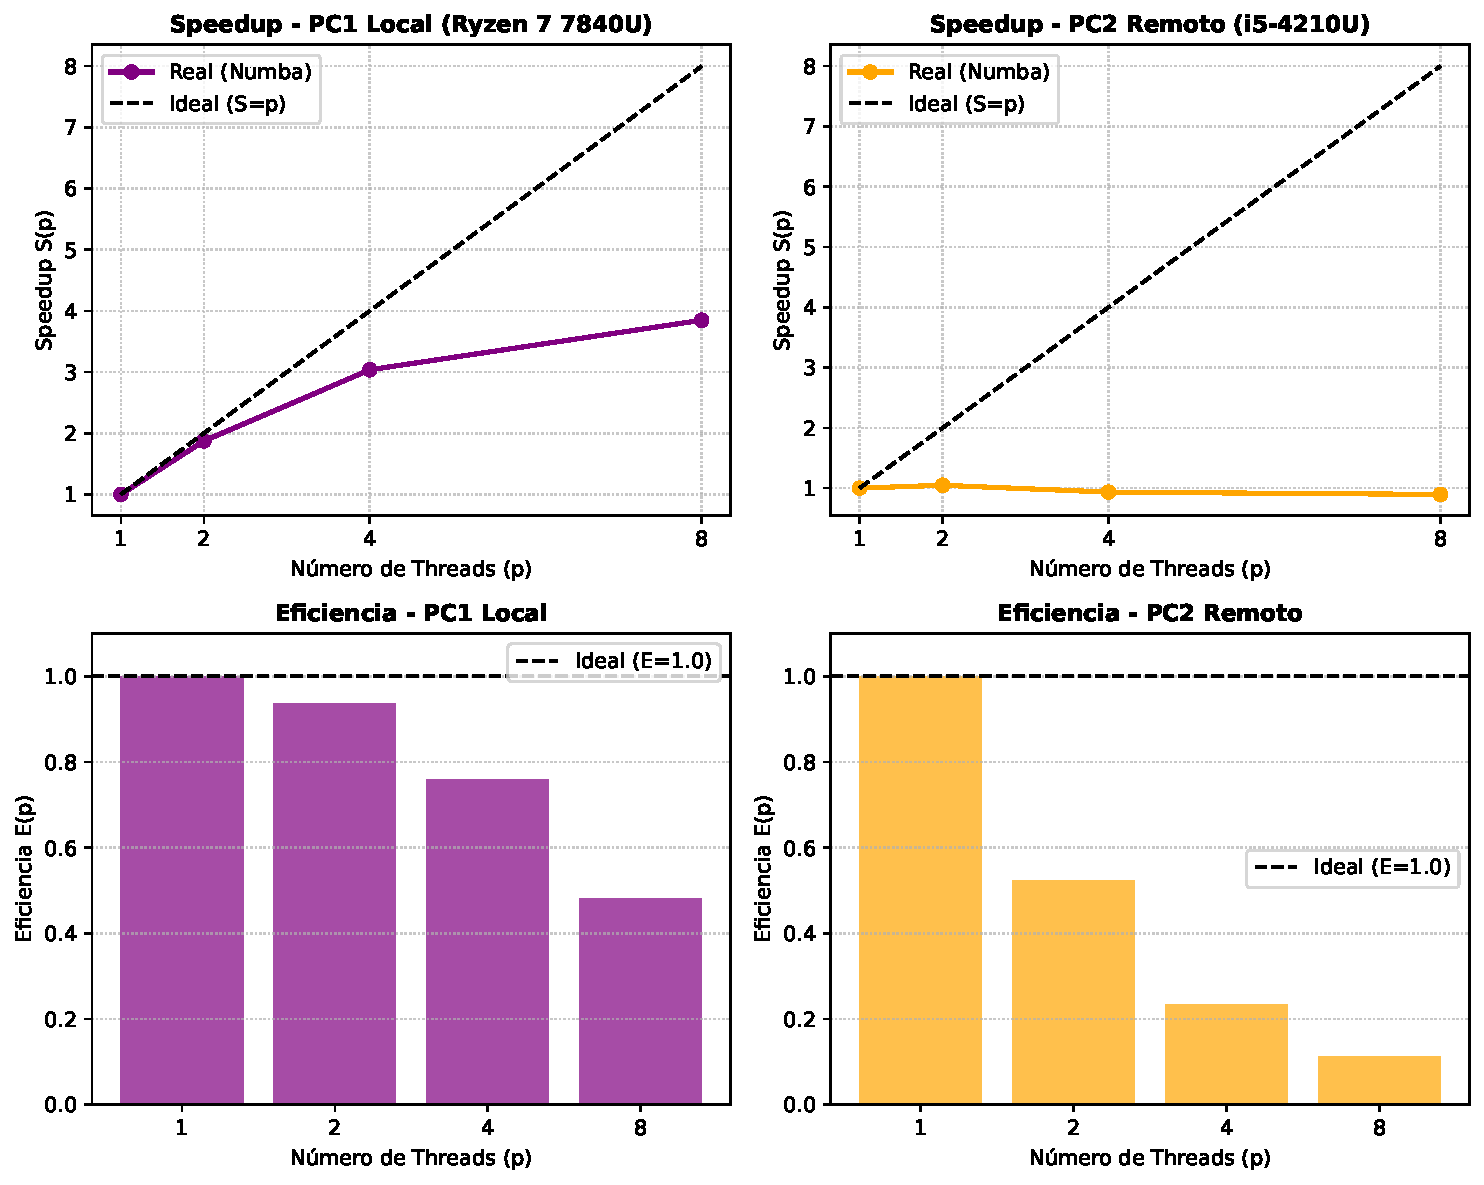
\includegraphics[width=\textwidth]{D/exp_d_plots.pdf}
    \caption{Resultados de Speedup y Eficiencia (Local vs. Remoto) para el Algoritmo 3 (Python con Numba).}
    \label{fig:exp_d_plots}
\end{figure}

\begin{table}[htbp]
\centering
\footnotesize
\setlength{\tabcolsep}{4pt}
\caption{Tiempos promedio (ms), Speedup $S(p)$ y Eficiencia $E(p)$ para el Algoritmo 3 (Numba, $N=2048$).}
\label{tab:resultados_d}
\begin{tabular}{r ccc ccc}
\toprule
& \multicolumn{3}{c}{\textbf{PC1 Local (AMD Ryzen 7 PRO 7840U)}} & \multicolumn{3}{c}{\textbf{PC2 Remoto (Intel Core i5-4210U)}} \\
\cmidrule(lr){2-4} \cmidrule(lr){5-7}
$p$ & Tiempo (ms) & Speedup $S(p)$ & Eficiencia $E(p)$ & Tiempo (ms) & Speedup $S(p)$ & Eficiencia $E(p)$ \\
\midrule
1 & 2014.47 & 1.0000 & 1.0000 & 5651.67 & 1.0000 & 1.0000 \\
2 & 1075.38 & 1.8733 & 0.9366 & 5394.04 & 1.0478 & 0.5239 \\
4 & 663.36  & 3.0368 & 0.7592 & 6052.48 & 0.9338 & 0.2334 \\
8 & 523.67  & 3.8468 & 0.4809 & 6308.52 & 0.8959 & 0.1120 \\
\bottomrule
\end{tabular}
\end{table}

\subsection{Comparación con las Otras Versiones}
En PC1, Numba demostró un rendimiento sobresaliente: a $p=1$ tomó \SI{2014.47}{\milli\second} frente a los \SI{4579.82}{\milli\second} del Algoritmo 1 en C++ con OpenMP (siendo más de $2\times$ más rápido), y a $p=8$ alcanzó \SI{523.67}{\milli\second} ($S(8)=3.85\times$). Esta ventaja frente al C++ ingenuo radica en la capacidad del optimizador LLVM de Numba para vectorizar eficientemente las operaciones sobre registros AVX2/FMA. Sin embargo, el Algoritmo 2 en C++ (dividir y conquistar con $n=256$) continúa siendo el más rápido con \SI{313.49}{\milli\second} a 8 hilos, confirmando que la reestructuración para el aprovechamiento de la memoria caché supera a la paralelización plana de filas.
